\documentclass[11pt]{ximera}  %Use handout to suppress answers
\usepackage{tikz}
\usepackage{amsmath}
\usetikzlibrary{arrows}
\usepackage{graphicx}
\usepackage{graphpap}
\usepackage{amssymb}
\usepackage{nicematrix}
\newcommand \Tstrut{\rule{0pt}{3ex}}   %Tstruct ensures the whole cell gets colored

\usepackage[nodisplayskipstretch]{setspace}
\usepackage{pgfplots}
\pgfplotsset{compat = newest}

\usepackage{xcolor-material} %For shark

%\usepackage{TikZlings}
\usepackage{tikzducks}
\newcommand{\owl}{\qedsymbol}

\usepackage{fontawesome5}

\usepackage{geometry}
\tikzset{%
    apple/.pic={
        \fill [MaterialBrown] (-1/8,0)
        arc (180:120:1 and 3/2) coordinate [pos=3/5] (@)-- ++(1/6,-1/7)
        arc (120:180:5/4 and 3/2) -- cycle;
        \fill [MaterialLightGreen500] (0,-9/10)
        .. controls ++(180:1/8) and ++(  0:1/4) .. (-1/3,  -1)
        .. controls ++(180:1/3) and ++(270:1/2) .. (  -1,   0)
        .. controls ++( 90:1/3) and ++(180:1/3) .. (-1/2, 3/4)
        .. controls ++(  0:1/8) and ++(135:1/8) .. (   0, 4/7)
        .. controls ++( 45:1/8) and ++(180:1/8) .. ( 1/2, 3/4)
        .. controls ++(  0:1/3) and ++( 90:1/3) .. (   1,   0)
        .. controls ++(270:1/2) and ++(  0:1/3) .. ( 1/3,  -1)
        .. controls ++(180:1/4) and ++(  0:1/8) .. cycle;
        \fill [MaterialLightGreen600] (0, 4/7)
        .. controls ++( 45:1/8) and ++(180:1/8) .. ( 1/2, 3/4)
        .. controls ++(  0:1/3) and ++( 90:1/3) .. (   1,   0)
        .. controls ++(270:1/2) and ++(  0:1/3) .. ( 1/3,  -1)
        .. controls ++(180:1/4) and ++(  0:1/8) .. (   0,-9/10);
        \fill [MaterialGreen500, shift={(@)}, rotate=-30]
        (0,0) arc (45:135:3/4 and 3/5) arc (225:315:3/4 and 3/5);
        \fill [MaterialGreen700, shift={(@)}, rotate=-30]
        (0,0) arc (315:225:3/4 and 3/5) -- cycle;
    }
}



\newcommand{\rulecolor}[1]{\def\CT@arc@{\color{#1}}}
\definecolor{darkblue}{rgb}{0.4,0.5,0.85}
\definecolor{blue}{rgb}{0.1,0.3,.95}
%\definecolor{blue}{rgb}{0.1,0.2,0.90}
\definecolor{pink}{rgb}{0.6,0.4,0.7}
\definecolor{green}{rgb}{0.4,0.6,0.5}
\definecolor{yellow}{rgb}{0.1,0.6,0.8}
\definecolor{red}{rgb}{0.8,0.1,0.5}
\definecolor{glaucous}{rgb}{0.38,0.51,0.71}

\usepackage{pgfplots}
\pgfplotsset{compat=1.16}
\usetikzlibrary{calc,angles,positioning,intersections,quotes,decorations.markings}
\pgfplotsset{soldot/.style={only marks,mark=*, line width=0.2pt, mark size=1.5pt}}
\pgfplotsset{holdot/.style={fill=white,only marks,mark=*, line width=1.0pt, mark size=1.5pt}}



\usepackage[utf8]{inputenc}  %needed to define \begin{axis} in tikz pic

\makeatletter
\renewcommand*\env@matrix[1][*\c@MaxMatrixCols c]{%
  \hskip -\arraycolsep
  \let\@ifnextchar\new@ifnextchar
  \array{#1}}
\makeatother

\setlength{\topmargin}{0cm} \setlength{\topskip}{0cm}
\setlength{\headheight}{0cm} \setlength{\headsep}{0cm}
\setlength{\oddsidemargin}{0cm} \setlength{\evensidemargin}{0cm}
\setlength{\footskip}{0cm} \setlength{\textwidth}{17.2cm}
\setlength{\textheight}{25cm}

\pagestyle{empty} \pagenumbering{none}


\title{Test Document - Take 101} \author{Kelly}

\begin{document}

\begin{abstract} Seeing if this thing works. \end{abstract} 
\maketitle

\begin{question}
A normal seated adult breathes in and exhales about $0.8$ L of air every $4$ seconds.  An experiment produced the graph below.  The volume $V$ of air
in the lungs $t$ seconds after exhaling can be approximated by a cosine function 
of the form $V= A \cos Bt + D,$   $0 \le t \le 8.$  Find the equation.    
%\textbf{Explain your reasoning and show your work.}  %Answer:  -0.35*cos(deg(pi*x/2)) + 0.45


\begin{center}
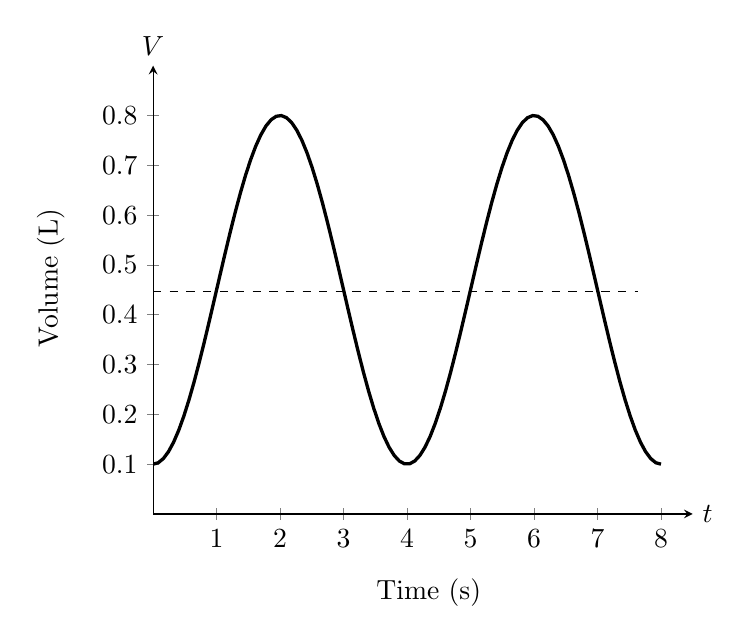
\begin{tikzpicture}
%\draw[help lines] (0,0) grid (8,8);
  \begin{axis} [axis lines=center, xmin = 0, xmax = 8.5, xtick={0, 1, 2, 3, 4, 5, 6, 7, 8},
    ymin = 0, ymax = 0.9, ytick={0, 0.1, 0.2, 0.3, 0.4, 0.5, 0.6, 0.7, 0.8}, xlabel={$t$}, ylabel={$V$}, every axis y label/.style={at=(current axis.above origin),anchor=south}, every axis x label/.style={at=(current axis.right of origin),anchor=west} ]
    \addplot [domain=0:8, samples=100, very thick] {-0.35*cos(deg(pi*x/2)) + 0.45};   %Can use smooth in place of samples = 100, but it makes graph chopy
  \end{axis}
  \node at (3.5,-1) {Time (s)};
  \node[rotate = 90] at (-1.3,3) {Volume (L)};
  \draw[dashed] (0,2.83)--(6.16,2.83);
\end{tikzpicture}
\end{center}

\begin{prompt}
\[
 V = \answer{-0.35\cos \left( \frac{\pi x}{2} \right) + 0.45} 
\]
\end{prompt}
\end{question} 



\begin{question}
What fraction of the circle is shaded?

 


%\begin{image}  %Makes circle huge!!  scale=0.1 does not help
\begin{center}
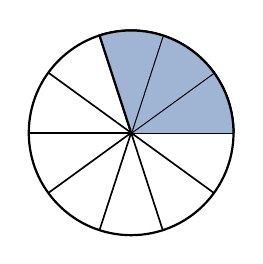
\begin{tikzpicture}
\draw[thick] (0,0) circle [radius=1.3cm];
\foreach \i in {36,72,...,360}
  \draw[semithick] (0,0)--(\i:1.3cm);    %The colon signifies that polar coordinates are being used. (60:.75cm) means the point that is at an angle of 60° and a distance of 0.75cm from the origin. Length of radial lines - should match radius above.


 \draw[thick, fill=glaucous!60] (0,0) --  (36:1.3) arc(36:0:1.3); %To Draw Arc: \draw (x,y) arc (start:stop:radius);

 \draw[thick, fill=glaucous!60] (0,0) --  (72:1.3) arc(72:36:1.3); %Colon indicates polar coordintes (angle:length)
 \draw[thick, fill=glaucous!60] (0,0) --  (108:1.3) arc(108:72:1.3);
% \draw[fill=glaucous] (0,0) -- (360:1.5) arc(360:324:1.5);

\end{tikzpicture}
\end{center}

\begin{multipleChoice}
\choice[correct]{$\displaystyle \frac{3}{10}$}
\choice{$\displaystyle \frac{1}{10}$}
\choice{$\displaystyle \frac{7}{10}$}
\end{multipleChoice}

\end{question}

\bigskip
%\begin{image}  Would not compile
\begin{center}
    \textbf{Maple Graph}\par\medskip
    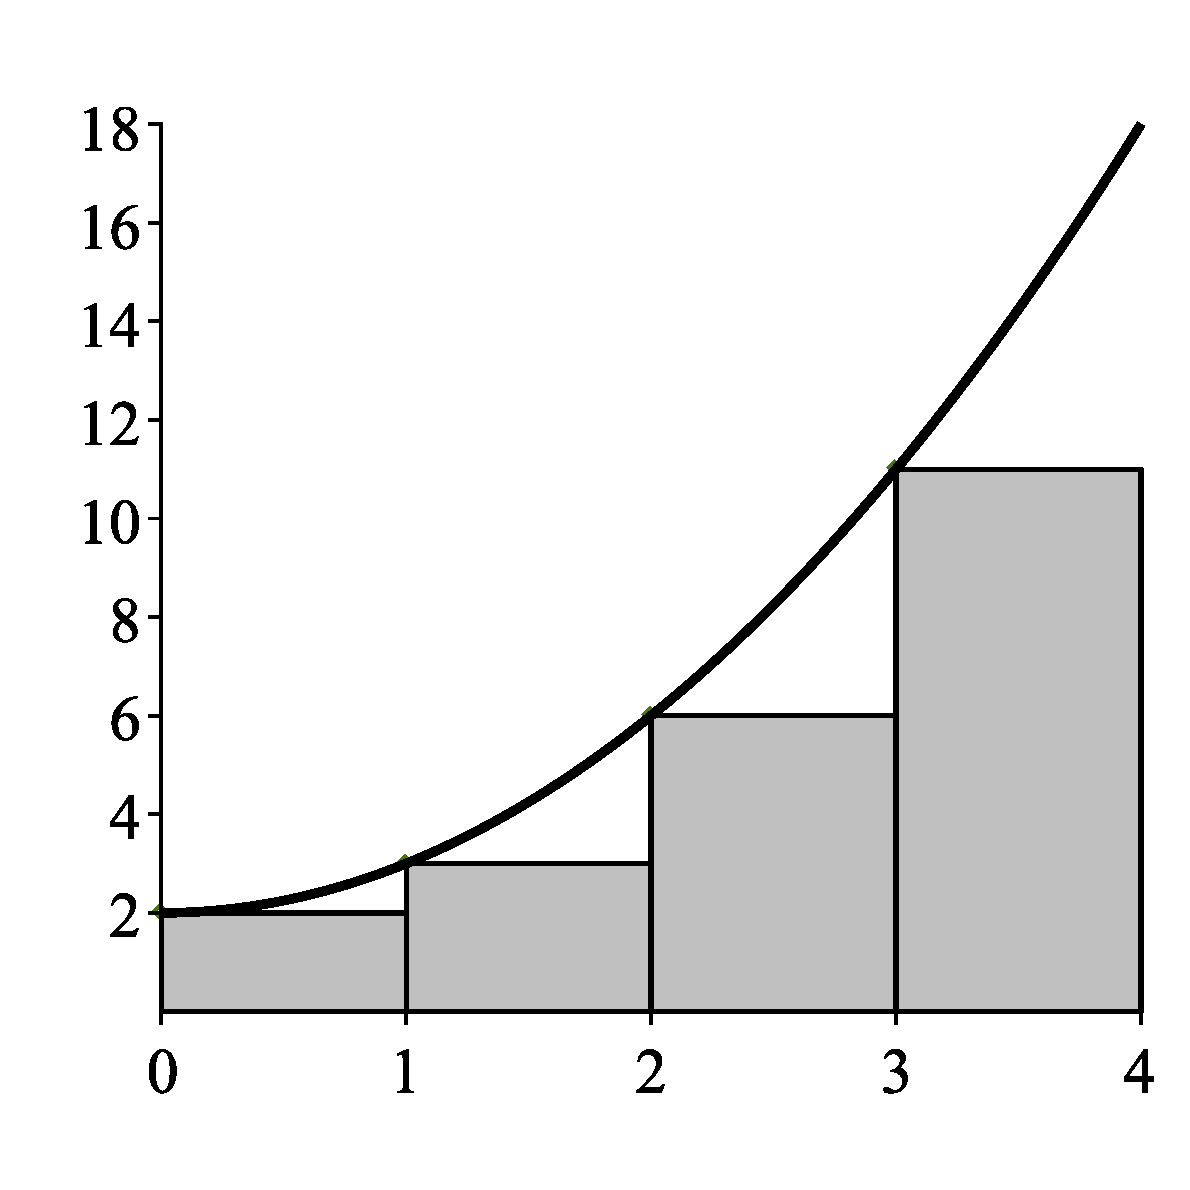
\includegraphics[scale=0.3]{reimannlo.eps}
    %\caption{Lower Sum}
\end{center}
%\end{image}

\begin{question}  
  $\lim_{x \rightarrow 3} x + 2 = \answer{5}$  
  \end{question}

\begin{question} 
$\lim\limits_{x\rightarrow 3} x + 2 =\answer{5} $
\end{question}

\end{document} 